\documentclass{standalone}
\usepackage[dvipsnames]{xcolor}
\usepackage{tikz}
\usetikzlibrary{math}
\usepackage{fontspec}

\tikzset{cardback/.pic={
	\begin{scope}
	\clip (-1.25in, 0in) --%
	      (-1.25in, 1.75in) --%
	      (1.25in, 1.75in) --%
	      (1.25in, -1.75in) --%
	      (-1.25in, -1.75in) --%
	      cycle;
	\foreach \i in {-1.25, -1.0,...,1.25}
		\foreach \j in {-1.75, -1.5, ..., 1.75}
			\draw[very thick, #1] (\i,\j) circle (0.105);

	\foreach \i in {-1.375, -1.125, -0.875,...,1.125, 1.375}
		\foreach \j in {-1.875, -1.625, ..., 1.875}
			\draw[very thick, #1] (\i,\j) circle (0.105);	
\end{scope}
	\node[draw, ultra thick, rounded corners=0.125in, inner sep=0pt, minimum height=3.5in, minimum width=2.5in] () at (0,0) {};
}}


\begin{document}
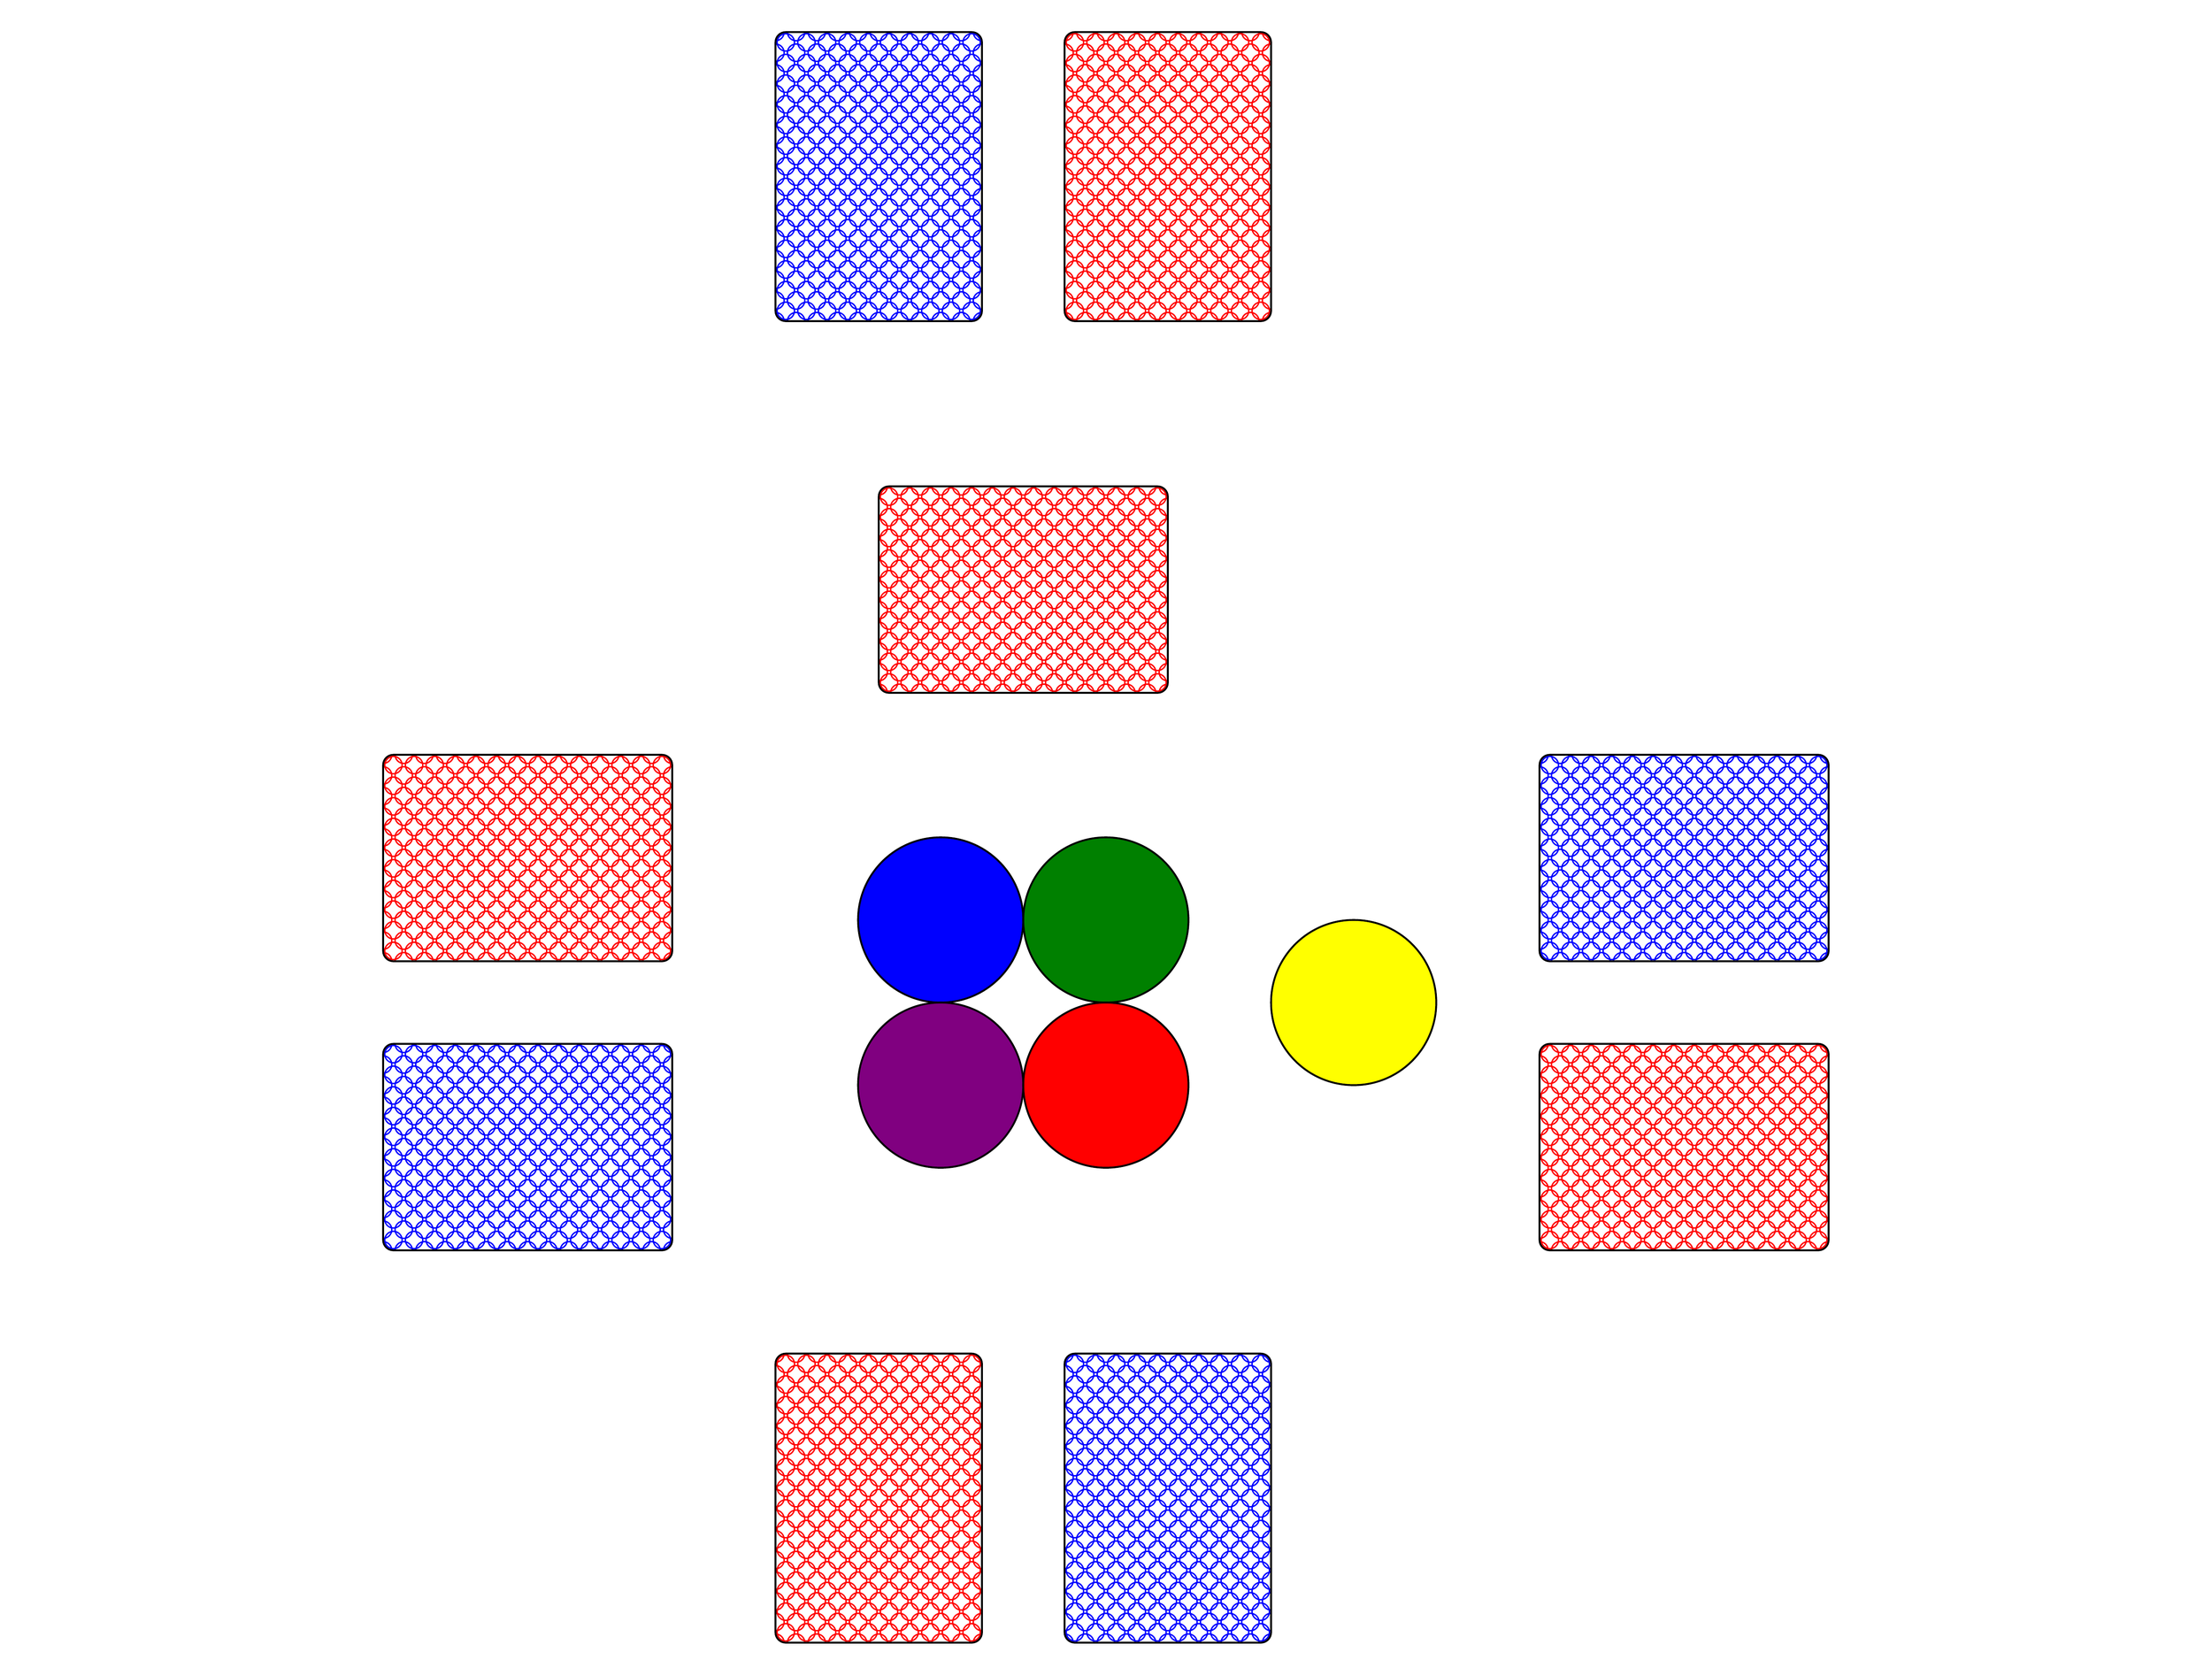
\begin{tikzpicture}[x=1in, y=1in, transform shape]
\path (-12.25, -8) to (14.25, 12);
\node[draw, circle, ultra thick, inner sep=0pt, minimum size=2in, fill=Blue] () at (-1,1) {};
\node[draw, circle, ultra thick, inner sep=0pt, minimum size=2in, fill=Green] () at (1,1) {};
\node[draw, circle, ultra thick, inner sep=0pt, minimum size=2in, fill=Purple] () at (-1,-1) {};
\node[draw, circle, ultra thick, inner sep=0pt, minimum size=2in, fill=Red] () at (1,-1) {};
\node[draw, circle, ultra thick, inner sep=0pt, minimum size=2in, fill=Yellow] () at (4,0) {};

\pic () at (-1.75,10) {cardback={Blue}};
\pic () at (1.75,10) {cardback={Red}};

\pic[rotate=90] at (8,1.75) {cardback={Blue}};
\pic[rotate=90] at (8,-1.75) {cardback={Red}};

\pic () at (-1.75,-6) {cardback={Red}};
\pic () at (1.75,-6) {cardback={Blue}};

\pic[rotate=90] at (-6,1.75) {cardback={Red}};
\pic[rotate=90] at (-6,-1.75) {cardback={Blue}};


\pic[rotate=90] at (0,5) {cardback={Red}};
\end{tikzpicture}
\end{document}
